\subsection[¿QUE ES UNA FSM?]{ ¿QUE ES UNA FSM?}
Una máquina de estados es un sistema secuencial sincrónico que posee un número fijo de posibles estados. El valor de sus salidas y la transición entre los estados depende del valor de sus entradas y del estado en que se encuentra actualmente. \textbf{Todos los cambios de estado ocurren ante un determinado flanco de la señal de reloj}(ya sea de subida o bajada).

Para entender mejor este concepto imaginemos que nuestra máquina de estados es un televisor, que sólo puede sintonizar cuatro canales y que se puede controlar por un control remoto que tiene solo dos teclas para aumentar o disminuir el canal. Los estados de nuestro sistema están representados por el número de canales que se pueden sintonizar, así pues, solo tendremos cuatro posibles estados (Número fijo de estados).  En la Figura 1 se muestra un diagrama de nuestro sistema:

{\centering 
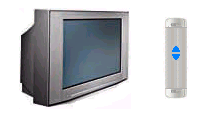
\includegraphics[width=5.715cm,height=3.122cm]{./images/FSM-img1.png} \par}

{\centering
Figura 1. Ejemplo de FSM.
\par}

Ahora hagámonos una pregunta: ¿Qué nos produce un cambio en el estado de nuestro sistema?, Lo único que nos puede producir un cambio de estado
(Canal sintonizado) es un cambio en las teclas de nuestro control remoto (Entradas del sistema). Observemos como actúa el sistema ante cambios de las entradas:

Si oprimimos la tecla de aumentar el canal, el televisor aumentará en uno la cadena sintonizada, por ejemplo, si estaba en el canal 1 pasará
al 2, si estaba en el 2 al 3, del 3 al 4 y del 4 al 1 nuevamente.

Si oprimimos la tecla menos es canal diminuirá pasando del 4 al 3, del 3 al 2, del 2 al 1 y del 1 al 4 nuevamente.
Si no oprimimos una tecla, el televisor debe permanecer en la cadena sintonizada actualmente y quedarse ahí hasta que se le ordene un cambio
por medio del control remoto.

Note que el estado (canal sintonizado) al que pasará el sistema depende del estado actual (canal actual) y de las entradas (tecla del control
remoto oprimida). Si las entradas no cambian el sistema no cambia su posición (esto no es necesariamente cierto para todas las máquinas de
estado).

\subsection[TABLAS Y DIAGRAMAS DE ESTADO]{TABLAS Y DIAGRAMAS DE ESTADO}

Existen varias formas de representar el comportamiento de las máquinas
de estado, siendo los más utilizados las tablas y los diagramas de
estado. Tomemos nuevamente el ejemplo del televisor y representemos en
una tabla los estados actual y siguiente (Estado al que pasa el sistema
ante un cambio de las entradas).

{\centering 
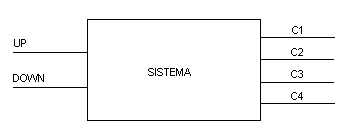
\includegraphics[width=9.206cm,height=3.651cm]{./images/FSM-img2.png} \par}

{\centering
Figura 2. Entradas y salidas del Sistema.
\par}

La Figura 2 muestra el sistema como una caja negra en la que sólo se indican las entradas y las salidas. Supongamos que nuestro sistema tiene dos entradas que son las correspondientes a Adelantar (UP) y disminuir (DN) canal, y que tiene cuatro salidas C1, C2, C3, C4 que corresponden a los cuatro canales y que me indican cual canal se está sintonizando actualmente. En este punto debemos tomar varias decisiones:

¿Cuando se considera que una entrada esta activa?, Es decir, con que valor lógico de la entrada se produce un cambio y con cual no. En nuestro caso un valor lógico alto en las entradas producirá un cambio de estado, es decir, si UP = {\textquoteleft}1{\textquoteright} el canal sintonizado aumentará o si DN = {\textquoteleft}1{\textquoteright} el canal disminuirá. Otra decisión que debemos tomar y que se deriva de esta es: que sucede si por error las dos entradas son {\textquoteleft}1{\textquoteright} simultáneamente, lo más conveniente es que el sistema conserve su estado ante esta posible situación.

El valor de las salidas para cada estado, en este ejemplo, un uno lógico en una salida indica que el canal ha sido seleccionado (por ejemplo, un
uno en C1 indicara que actualmente el canal seleccionado es el 1), por lo tanto sólo una salida puede tener un valor lógico alto.

Una vez definido completamente el funcionamiento de nuestro sistema se procede  a representarlo mediante una tabla de estados:

\subsubsection[Tabla de Estados]{ Tabla de Estados}
{\centering 
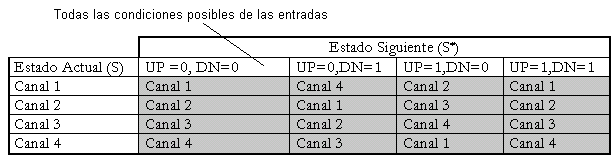
\includegraphics[width=14.991cm,height=3.895cm]{./images/FSM-img3.png} \par}

{\centering
Figura 3. Tabla de estados del sistema Televisor.
\par}

La Figura 3. Muestra una tabla de estados típica en la cual se resume el comportamiento del sistema. La tabla tiene tres secciones: El estado actual: Lista de todos lo posibles estados.

Posibles combinaciones de las entradas: El número de entradas del sistema determina el número de columnas de la tabla de estados. Así, si la máquina tiene n entradas, la tabla tendrá 2\textsuperscript{n} +1 Columnas.

El estado siguiente: Indica a que estado pasará la FSM cuando se presente una determinada entrada, Por ejemplo, Si UP=0 y DOWN = 1 y el estado actual es el canal 4 la máquina de estados irá al estado Canal 3.

Otra forma de representar el estado de las entradas es utilizando una convención en la que si la variable aparece negada entonces toma un valor de cero lógico, pero si no lo esta tiene un valor de uno lógico. Esto se hace para simplificar las tablas. Por ejemplo:


A:\ \ A = {\textquoteleft}1{\textquoteright}

{!A:\ \ A = 0;}

Con lo que la tabla de estados se convierte en :

\begin{center}
\tablehead{}
\begin{supertabular}{|m{2.441cm}|m{1.8739998cm}|m{1.68cm}|m{1.68cm}|m{1.486cm}|m{2.3309999cm}|}
\hline &
\multicolumn{4}{m{7.32cm}|}{\centering  Estado Siguiente} &
\centering\arraybslash  Salidas\\\hline
\centering  Estado Actual &
\centering  !UP.!DN &
\centering  !UP.DN &
\centering  UP.!DN &
\centering  UP.DN &
\centering\arraybslash  C1,C2,C3,C4\\\hline
\centering  Canal 1 &
\centering  Canal 1 &
\centering  Canal 4 &
\centering  Canal 2 &
\centering  Canal 1 &
\centering\arraybslash  1,0,0,0\\\hline
\centering  Canal 2 &
\centering  Canal 2 &
\centering  Canal 1 &
\centering  Canal 3 &
\centering  Canal 2 &
\centering\arraybslash  0,1,0,0\\\hline
\centering  Canal 3 &
\centering  Canal 3 &
\centering  Canal 2 &
\centering  Canal 4 &
\centering  Canal 3 &
\centering\arraybslash  0,0,1,0\\\hline
\centering  Canal 4 &
\centering  Canal 4 &
\centering  Canal 3 &
\centering  Canal 1 &
\centering  Canal 4 &
\centering\arraybslash  0,0,0,1\\\hline
\end{supertabular}
\end{center}
{\centering
Tabla 1. Tabla de Estados del sistema Televisor.
\par}

\subsubsection[Diagrama de Estados]{ Diagrama de Estados}

Otra forma de representar el comportamiento de una máquina de estados es el diagrama de estados, este diagrama es una representación gráfica del
funcionamiento del sistema. 

 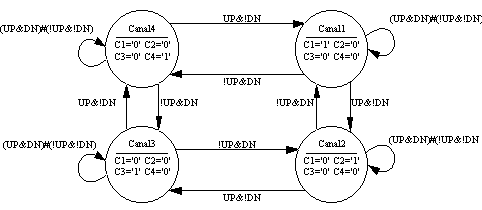
\includegraphics[width=12.751cm,height=5.556cm]{./images/FSM-img4.png}

{\centering Figura 4. Diagrama de estados del sistema Televisor. \par}

La Figura 4 muestra el diagrama de bloques del sistema televisor. Observamos que cada estado está representado por un círculo en el que se indica el nombre del mismo y el valor de las salidas. Las líneas que unen los estados representan el cambio que sufre la máquina cuando se cumple una determinada regla de transición. (La regla de transición normalmente se indican en las líneas que unen los estados). En esta figura se introduce una nueva nomenclatura para representar las funciones lógicas, el operador \textbf{\textit{not}} se representa con el signo \textbf{\textit{!}}, la operación \textbf{\textit{AND}} con el signo \textbf{\textit{\&}} y la \textbf{\textit{OR}} con \textbf{\textit{\#}}.

Podemos observar que del estado Canal1, salen dos líneas: Una hacia el estado Canal2, lo que indica que la máquina pasará de Canal1 a Canal2 si UP = {\textquoteleft}1{\textquoteright} y DN = {\textquoteleft}0{\textquoteright} y se presenta un flanco adecuado en
la señal de reloj; Otra hacia el estado Canal4, lo que indica que la máquina de estados pasará de Canal1 a Canal4 si UP = {\textquoteleft}0{\textquoteright},  DN = {\textquoteleft}1{\textquoteright} y se presenta un flanco adecuado en la señal de reloj.

Así mismo tenemos dos líneas que llegan al Estado Canal1: Una proviene del estado Canal2, con lo que el sistema pasará de Canal2 a Canal 1 si UP = {\textquoteleft}0{\textquoteright}, DN = {\textquoteleft}1{\textquoteright} y se presenta un flanco adecuado en la señal de reloj; y otra desde el estado Canal4. lo que hace que el sistema pase de Canal4 a Canal 1 si UP = {\textquoteleft}1{\textquoteright} y DN = {\textquoteleft}0{\textquoteright} y se presenta un flanco adecuado en la señal de reloj.

Por último existe una curva que sale del Canal1 y vuelve a entrar a Canal1, esto indica que la máquina mantendrá su estado si: (UP 
= {\textquoteleft}0{\textquoteright} Y DN = {\textquoteleft}0{\textquoteright} ) O (UP = {\textquoteleft}1{\textquoteright} Y DN = {\textquoteleft}1{\textquoteright}).

\subsection[SINTESIS DE FSM]{ SINTESIS DE FSM}

En esta sección analizaremos la arquitectura de la FSM y el proceso de síntesis. Como vimos en el capítulo anterior la síntesis parte de una descripción funcional y llega a una descripción a nivel de compuertas.

 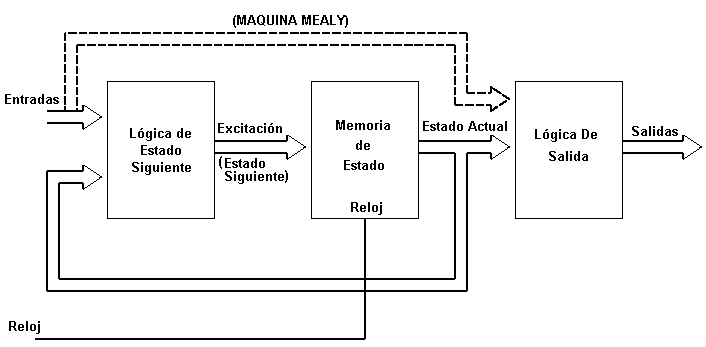
\includegraphics[width=12.27cm,height=6.04cm]{./images/FSM-img5.png} 

{\centering Figura 5. Estructura de una FSM. \par}

\subsubsection[Estructura de una FSM]{ Estructura de una FSM}
La estructura general de una máquina de estados se muestra en la  Figura 5. Como puede observarse existen tres bloques bien definidos:

Lógica de estado siguiente: Está encargada de generar las señales necesarias para producir un cambio de estado en la FSM (Estado Siguiente). Puede observarse que el estado siguiente depende del estado actual y de las entradas 

Memoria de Estado: Normalmente esta formada por Flip-Flops tipo D o JK, los cuales tienen la misma señal de reloj. Las salidas de los Flip-Flops determinan el estado actual de la FSM, cada salida del Flip-Flop puede tomar dos valores distintos {\textquoteleft}1{\textquoteright} o
{\textquoteleft}0{\textquoteright}, por lo tanto se pueden tener dos estados con un Flip-Flop. Si tenemos N Flip-Flops tendremos 2\textsuperscript{N} estados.

Lógica de Salida: La lógica de salida esta encargada de producir los valores necesarios a la salida de la FSM, su la arquitectura esta basada en decodificadores. 

Existen dos tipos de máquinas de estados: Moore: El estado siguiente depende del valor de las entradas y del estado actual; Y la salida depende únicamente del estado actual; y Mealy: Al igual que la máquina de Moore el estado siguiente depende del valor de las entradas y del estado actual, pero se diferencian en que la salida depende del estado actual y del valor de las entradas.

\subsubsection[Proceso de Síntesis]{ Proceso de Síntesis}

El primer paso en el proceso de síntesis de una FSM y en general de cualquier sistema digital es la descripción del sistema ya sea mediante
un algoritmo o de un diagrama de tiempos. El siguiente paso consiste en pasar la descripción funcional a un diagrama de estados para su posterior representación en tablas de estado y de salida. A continuación debemos reducir el número de estados (si es posible) utilizando algoritmos de minimización. Después debemos realizar la codificación de estados, es decir, asignarle a los estados un grupo único de valores que corresponden a los valores que tomarán los Flip-Flops. A continuación se debemos obtener las ecuaciones de estado siguiente y de salidas. El siguiente paso consiste en la elección del tipo de Flip-Flop que se va a utilizar para la implementación, recuerde que todos los Flip\_Flops tienen diferentes ecuaciones de estado siguiente:

\begin{center}
\tablehead{}
\begin{supertabular}{|m{2.142cm}|m{3.61cm}|}
\hline
\centering  Tipo de F-F &
\centering\arraybslash  Estado Siguiente
(Q\textsuperscript{*})\\\hline
\centering  D &
\centering\arraybslash  Q* = D\\\hline
\centering  JK &
\centering\arraybslash  Q* = J,!Q + !K.Q\\\hline
\centering  T &
\centering\arraybslash  Q* = !Q\\\hline
\centering  SR &
\centering\arraybslash  Q* = S + !R.Q\\\hline
\end{supertabular}
\end{center}

{\centering Tabla 2. Ecuaciones de Estado siguiente de los Flip-Flop. \par}

Una vez elegido el Flip-Flop se procede a obtener las ecuaciones de las señales de excitación de los FFs. Después se de be realizar un proceso
de minimización con las ecuaciones obtenidas anteriormente para realizar un diagrama de la implementación lógica de las ecuaciones. Finalmente debemos verificar el correcto funcionamiento del circuito, esto se logra simulando el circuito obtenido y si cumple con lo requerimientos se llevará al plano físico para realizar pruebas de tiempos. La figura 6 resume los pasos a seguir en el proceso de síntesis.

{\centering 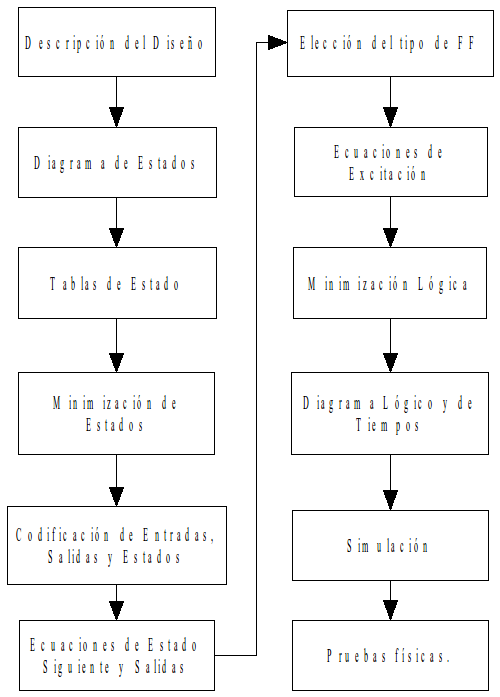
\includegraphics[width=9.135cm,height=12.734cm]{./images/FSM-img6.png} \par}

{\centering Figura 6. Diagrama de flujo del proceso de Síntesis para FSM \par}

Para entender mejor el proceso de síntesis realizaremos paso a paso un sencillo ejemplo. Desarrollando todas las posibilidades de implementación para buscar la más óptima.

\subsubsection[Control de Motor de Paso.]{Control de Motor de Paso.}

Un motor de paso a diferencia de los motores de Corriente Continua necesita una secuencia determinada en sus cuatro terminales para originar el giro de su rotor. La secuencia necesaria para controlar el motor es la siguiente:

\begin{center}
\tablehead{}
\begin{supertabular}{|m{2.679cm}|m{2.892cm}|m{2.892cm}|m{2.892cm}|m{2.945cm}|}
\hline
 &
\centering  A & \centering  B & \centering  C & \centering\arraybslash  D\\\hline
\centering  S1 & \centering  V+ & \centering  GND & \centering  V+ & \centering\arraybslash  GND\\\hline
\centering  S2 & \centering  V+ & \centering  GND & \centering  GND & \centering\arraybslash  V+\\\hline
\centering  S3 & \centering  GND & \centering  V+ & \centering  GND & \centering\arraybslash  V+\\\hline
\centering  S4 & \centering  GND & \centering  V+ & \centering  V+ & \centering\arraybslash  GND\\\hline
\end{supertabular}
\end{center}
Para que el motor gire un paso (normalmente 1.8 grados) es necesario que se aplique S1 y luego S2, o S2 y S3 o S3 y S4 o S4 y S1. Si se desea que el motor gire cinco pasos se debe seguir la secuencia S1, S2, S3, S4, S5. La inversión del sentido de giro se logra invirtiendo la secuencia anterior, es decir, S1, S4, S3, S2, S1.

\paragraph[Diagrama de Caja Negra]{Diagrama de Caja Negra}

El primer paso consiste en realizar un diagrama de caja negra en el que se indiquen las entradas y salidas (Figura 7).

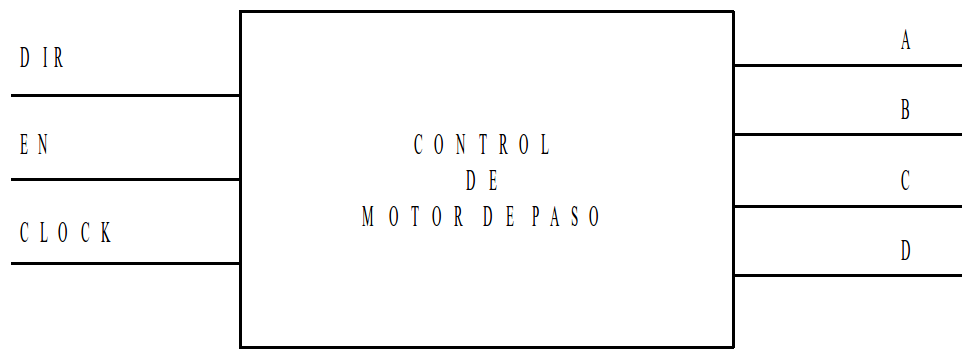
\includegraphics[width=11.023cm,height=4.064cm]{./images/FSM-img7.png} 
Figura 7. Diagrama de Caja Negra del Controlador de Motor de Paso.

A continuación realizaremos una breve descripción del funcionamiento del circuito. Como se observa en la Figura 7. Se tienen tres entradas:

DIR: Encargada de indicar la dirección de giro del motor. DIR = 0 Secuencia Directa (S1, S2, S3, S4), DIR = 1 Secuencia Invertida (S4, S3, S2, S1)
EN: ENABLE, encargada de habilitar nuestro control Si EN = 1 el circuito realizará su función si EN = 0 el control conservará el último estado
de las salidas. 

CLOCK: Es el reloj del sistema y gobierna todas las transiciones entre estados. 
Y las cuatro salidas A, B, C, D son las encargadas de manejar los terminales del motor de paso.

\paragraph[Diagrama de Estado]{ Diagrama de Estado}

Una vez se conoce el funcionamiento del circuito, o las funciones que debe cumplir se procede a realizar el diagrama de estados del mismo. La
Figura 8 muestra este diagrama para el controlador de motor de paso.

{\centering 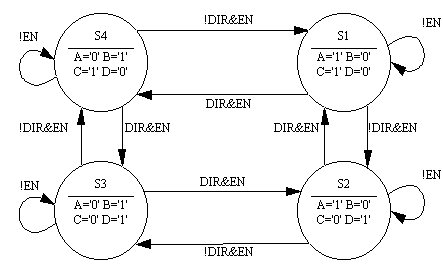
\includegraphics[width=11.719cm,height=7.142cm]{./images/FSM-img8.png} \par}
Figura 8 Diagrama de Estados del Controlador de Motor de Paso.

\paragraph[Tabla de estados]{ Tabla de estados}

Una vez realizado el diagrama de estados se procede a la realización de la tabla de estados y salidas. Dicha tabla para el controlador de motor
de paso se presente a continuación:

\begin{center}
\tablehead{}
\begin{supertabular}{|m{2.5379999cm}|m{1.798cm}|m{1.714cm}|m{1.714cm}|m{1.629cm}|m{1.9549999cm}|}
\hline  &
\multicolumn{4}{m{7.4550004cm}|}{\centering 
Estado Siguiente} &
\centering\arraybslash  Salidas\\\hline
\centering  Estado Actual &
\centering  !EN.!DIR &
\centering  !EN.DIR &
\centering  EN.!DIR &
\centering  EN.DIR &
\centering\arraybslash  A, B, C, D\\\hline
\centering  S1 &
\centering  S1 &
\centering  S1 &
\centering  S2 &
\centering  S4 &
\centering\arraybslash  1, 0, 1, 0\\\hline
\centering  S2 &
\centering  S2 &
\centering  S2 &
\centering  S3 &
\centering  S1 &
\centering\arraybslash  1, 0, 0, 1\\\hline
\centering  S3 &
\centering  S3 &
\centering  S3 &
\centering  S4 &
\centering  S2 &
\centering\arraybslash  0, 1, 0, 1\\\hline
\centering  S4 &
\centering  S4 &
\centering  S4 &
\centering  S1 &
\centering  S3 &
\centering\arraybslash  0, 1, 1, 0\\\hline
\end{supertabular}
\end{center}

\paragraph[Minimización de Estados]{Minimización de Estados}

El objetivo de la minimización de estados es la reducción del número de Flip-Flops necesarios para la implementación, reduciendo de este modo el costo de la misma. Sin embargo para reducir el número de Flip-Flops de un circuito es necesario reducir el número de estados en múltiplos de 2. Por ejemplo, supongamos que tenemos 7 estados, para lo cual necesitamos 3 FFs, para utilizar sólo 2 FFs necesitamos reducir el número de estados de 7 a 4 o menos.

La minimización de estados se basa en la equivalencia funcional, por ejemplo, se dice que dos circuitos son equivalentes cuando proporcionan la misma salida ante los mismos cambios de entrada. Dos o más estados son equivalentes sí:

Ambos estados producen las mismas salidas ante igual cambio en las señales de entrada.
Ambos estados tienen los mismos estados siguientes ante los mismos cambios de las señales de entrada.

En nuestro caso no tenemos equivalentes ya que todos tienen diferentes valores de salida y diferentes estados siguientes ante variaciones de
las entradas.

\paragraph[Codificación de estados]{Codificación de estados}
La codificación de estados consiste en la asignación de valores a las salidas de los FFs para cada estado, estos valores deben ser únicos para cada estado, es decir, no se deben repetir. Debido a que nuestra máquina tiene cuatro estados, tenemos 2 FFs y por lo tanto debemos asignar a cada estado un código formado por dos bits. Existen muchas posibles codificaciones para los cuatro estados, unas más eficientes que otras. En este libro no se tratarán las técnicas existentes para hallar la codificación óptima ya que esta función las realizan las herramientas CAD y además, se sale del objetivo de este libro. Para nuestro ejemplo utilizaremos la siguiente codificación:

\begin{center}
\tablehead{}
\begin{supertabular}{|m{0.67800003cm}|m{0.791cm}|m{0.84400004cm}|}
\hline  &
\centering  Q1 & \centering\arraybslash  Q0\\\hline 
\centering  S1 & \centering  0 & \centering\arraybslash  0\\\hline
\centering  S2 & \centering  0 & \centering\arraybslash  1\\\hline
\centering  S3 & \centering  1 & \centering\arraybslash  0\\\hline
\centering  S4 & \centering  1 & \centering\arraybslash  1\\\hline
\end{supertabular}
\end{center}

Donde Q1 y Q0 son las salidas del primer y segundo FF correspondientemente. Con esta asignación de estados la tabla de estados queda de la siguiente forma:

\begin{center}
\tablehead{}
\begin{supertabular}{|m{0.791cm}|m{0.791cm}|m{0.897cm}|m{0.897cm}|m{0.897cm}|m{0.897cm}|m{0.897cm}|m{0.897cm}|m{1.98cm}|}
\hline
\multicolumn{2}{|m{1.782cm}|}{\centering {Estado Actual}\par
\centering  (S)} &
\multicolumn{6}{m{6.3820004cm}|}{\centering 
Estado Siguiente (S\textsuperscript{*})} &
\centering\arraybslash 
SALIDAS\\\hhline{~~------~}
 &  &
\multicolumn{2}{m{1.994cm}|}{\centering  !EN} &
\multicolumn{4}{m{4.188cm}}{\centering  EN} &
\\\hhline{~~-------}  &  &  &  &
\multicolumn{2}{m{1.994cm}|}{\centering  !DIR} &
\multicolumn{2}{m{1.994cm}|}{\centering  DIR} &
\centering\arraybslash  A, B, C, D\\\hline
\centering  Q1 & \centering  Q0 & 
\centering  Q1\textsuperscript{*} &
\centering  Q0\textsuperscript{*} &
\centering  Q1\textsuperscript{*} &
\centering  Q0\textsuperscript{*} &
\centering  Q1\textsuperscript{*} &
\multicolumn{1}{m{0.897cm}}{\centering 
Q0\textsuperscript{*}} &
\\\hline
\centering  0 & \centering  0 & \centering  0 & \centering  0 & \centering  0 & \centering  1 & \centering  1 & \centering  1 &
\centering\arraybslash  1, 0, 1, 0\\\hline
\centering  0 & \centering  1 & \centering  0 & \centering  1 & \centering  1 & \centering  0 & \centering  0 & \centering  0 &
\centering\arraybslash  1, 0, 0, 1\\\hline 
\centering  1 & \centering  0 & \centering  1 & \centering  0 & \centering  1 & \centering  1 & \centering  0 & \centering  1 &
\centering\arraybslash  0, 1, 0, 1\\\hline
\centering  1 & \centering  1 & \centering  1 & \centering  1 & \centering  0 & \centering  0 & \centering  1 & \centering  0 &
\centering\arraybslash  0, 1, 1, 0\\\hline
\end{supertabular}
\end{center} 


Donde Q1\textsuperscript{*} y Q0\textsuperscript{*} representan los valores siguientes de las señales Q1 y Q0 respectivamente. Note que no
se representaron los casos !EN.!DIR y !EN.DIR, esto se debe a que cuando la señal En tiene un valor lógico bajo la FSM conserva su estado
sin importar el valor de DIR.

\paragraph[Ecuaciones de estado siguiente]{Ecuaciones de estado siguiente}

Una vez realizada la codificación de estados se procede a la obtención de las ecuaciones de estado siguiente Q1\textsuperscript{*} y  Q0\textsuperscript{*}. Para obtener estas ecuaciones debemos sumar todos los unos de la tabla de estados (suma de minitérminos). Para Q1\textsuperscript{*} debemos observar todas las columnas correspondientes a Q1\textsuperscript{*} y sumar los minitérminos asociados. Por ejemplo, la primera columna de Q1* correspondiente a la asociada con !EN, el primer minitérmino asociado es: !EN.Q1.!Q0 ya que está en la fila correspondiente a Q1 = 1 y Q0 = 0. Y el segundo !EN.Q1.Q0. \\

{Q1\textsuperscript{*} = !EN.Q1.!Q0 + !EN.Q1.Q0 + EN.!DIR.!Q1.Q0 + EN.!DIR.Q1.!Q0 + EN.DIR.!Q1.!Q0 + EN.DIR.Q1.Q0.\\
Q0\textsuperscript{*} = !EN.!Q1.Q0 + !EN.Q1.Q0 + EN.!DIR.!Q1.!Q0 + EN.!DIR.Q1.!Q0 + EN.DIR.!Q1.!Q0 + EN.DIR.Q1.!Q0.}

Estas ecuaciones deben pasar a través de un proceso de minimización para encontrar una implementación óptima.

Q1* = !EN.Q1(!Q0+Q1) + EN.(!DIR.(!Q1.Q0 + Q1.!Q0) + DIR (!Q1.!Q0 + Q1.Q0)) \\
Q1* = !EN.Q1 + EN.(!DIR.Q1 Q0 + DIR.!(Q1 Q0)) \\
Q1* = !EN.Q1 + EN.DIR (Q1 XOR Q0) \\
Q0* = !EN.Q0.(!Q1 + Q1) + EN.(!Q1.!Q0.(!DIR + DIR) + Q1.!Q0.(!DIR + DIR)) \\
Q0* = !EN.Q0 + EN.(!Q1.!Q0 + Q1.!Q0) \\
Q0* = !EN.Q0 + EN.(!Q0.(!Q1+ Q1)) \\
Q0* = !EN.Q0 + EN.!Q0 \\
Q0* = EN XOR Q0 \\

Las ecuaciones para las salidas son:

{A = !Q1.!Q0 + !Q1.Q0 = !Q1}
{B = Q1.!Q0 + Q1.Q0 = Q1}
{C = !Q1.!Q0 + Q1.Q0 = !(Q1 Q0)}
{D = !Q1.Q0 + Q1.!Q0 = Q1 Q0}
{A = !B = !Q1}
{C = !D = Q1 XOR Q0}

\paragraph[Elección del tipo de Flip{}-Flop, ecuaciones de excitación y minimización]{ Elección del tipo de Flip-Flop, ecuaciones de excitación y minimización}

Utilizando las ecuaciones obtenidas anteriormente para Q1* y Q0*, debemos escoger el tipo de Flip-Flop a utilizar. La siguiente tabla resume los valores necesarios en las entradas de los FFs para obtener los cambios indicados en sus salidas. Por ejemplo en un FF JK si Q tiene un valor de 0 lógico y se quiere que pase a tener un valor de 1 lógico es necesario que J = 1 y el valor de K no importa.

\begin{center}
\tablehead{}
\begin{supertabular}{|m{1.2689999cm}|m{0.95699996cm}|m{0.95699996cm}|m{0.55cm}|m{0.663cm}|}
\hline
\centering  Q  Q* & \centering  S  R & \centering  J  K & \centering  T & \centering\arraybslash  D\\\hline
\centering  0  0 & \centering  0  X & \centering  0  X & \centering  0 & \centering\arraybslash  0\\\hline
\centering  0  1 & \centering  1  0 & \centering  1  X & \centering  1 & \centering\arraybslash  1\\\hline
\centering  1  0 & \centering  0  1 & \centering  X  1 & \centering  1 & \centering\arraybslash  0\\\hline
\centering  1  1 & \centering  X  0 & \centering  X  0 & \centering  0 & \centering\arraybslash  1\\\hline
\end{supertabular}
\end{center}

El diagrama de Karnough para la máquina de estados es el siguiente

\begin{center}
\tablehead{}
\begin{supertabular}{|m{0.675cm}|m{0.772cm}|m{0.772cm}|m{0.772cm}|m{0.825cm}|}
\hline  &
\centering  00 & \centering  01 & \centering  11 & \centering\arraybslash  10\\\hline
\centering  00 & \centering  \textbf{0} 0 & \centering  \textbf{0} 0 & \centering  \textbf{1} 1 & \centering\arraybslash  \textbf{0} 1\\\hline
\centering  01 & \centering  \textbf{0} 1 & \centering  \textbf{0} 1 & \centering  \textbf{0} 0 & \centering\arraybslash  \textbf{1} 0\\\hline
\centering  11 & \centering  \textbf{1} 1 & \centering  \textbf{1} 1 & \centering  \textbf{1} 0 & \centering\arraybslash  \textbf{0} 0\\\hline
\centering  10 & \centering  \textbf{1} 0 & \centering  \textbf{1} 0 & \centering  \textbf{0} 1 & \centering\arraybslash  \textbf{1} 1\\\hline
\end{supertabular}
\end{center}

La región sombreada corresponde a los valores de las señales Q1* (en negrilla) y Q0*.


Para el FF D tenemos: Q* = D. Por lo tanto:
 
{D1 = !EN.Q1 + EN.DIR (Q1 XOR Q0)}
{D0 = EN XOR Q0}

Para el FF JK debemos ordenar las ecuaciones obtenidas de la forma: Q* =J.!Q + !K.Q, por lo que para Q1:

\begin{center}
\tablehead{}
\begin{supertabular}{|m{0.675cm}|m{0.95699996cm}|m{0.95699996cm}|m{0.95699996cm}|m{1.01cm}|}
\hline  &
\centering  00 & \centering  01 & \centering  11 & \centering\arraybslash  10\\\hline
\centering  00 & \centering  \textbf{0}  X & \centering  \textbf{0}  X & \centering  \textbf{1}  X & \centering\arraybslash  \textbf{0}  X\\\hline
\centering  01 & \centering  \textbf{0}  X & \centering  \textbf{0}  X & \centering  \textbf{0}  X & \centering\arraybslash  \textbf{1}  X\\\hline
\centering  11 & \centering  \textbf{X}  0 & \centering  \textbf{X}  0 & \centering  \textbf{X}  0 & \centering\arraybslash  \textbf{X}  1\\\hline
\centering  10 & \centering  \textbf{X}  0 & \centering  \textbf{X}  0 & \centering  \textbf{X}  1 & \centering\arraybslash  \textbf{X}  0\\\hline
\end{supertabular}
\end{center}

La región sombreada indican los valores que deben tener las señales J1(en negrilla) y K1.
{J1 = !Q1.!Q0.EN.DIR + !Q1.Q0.EN.!DIR = EN.!Q1(Q0 XOR DIR)}
{K1 = Q1.!Q0.EN.DIR + Q1.Q0.EN.!DIR = EN.Q1.(Q0 XOR DIR)}

Para Q0

\begin{center}
\tablehead{}
\begin{supertabular}{|m{0.675cm}|m{0.95699996cm}|m{0.95699996cm}|m{0.95699996cm}|m{1.01cm}|}
\hline  &
\centering  00 & \centering  01 & \centering  11 & \centering\arraybslash  10\\\hline
\centering  00 & \centering  \textbf{0}  X & \centering  \textbf{0}  X & \centering  \textbf{1}  X & \centering\arraybslash  \textbf{1}  X\\\hline
\centering  01 & \centering  \textbf{X}  0 & \centering  \textbf{X}  0 & \centering  \textbf{X}  1 & \centering\arraybslash  \textbf{X}  1\\\hline
\centering  11 & \centering  \textbf{X}  0 & \centering  \textbf{X}  0 & \centering  \textbf{X}  1 & \centering\arraybslash  \textbf{X}  1\\\hline
\centering  10 & \centering  \textbf{0}  X & \centering  \textbf{0 } X & \centering  \textbf{1}  X & \centering\arraybslash  \textbf{1}  X\\\hline
\end{supertabular}
\end{center}

{J0 = EN}
{K0 = EN}

{Flip-Flop tipo T:}

{Para Q1:}

\begin{center}
\tablehead{}
\begin{supertabular}{|m{0.675cm}|m{0.772cm}|m{0.772cm}|m{0.772cm}|m{0.825cm}|}
\hline&
\centering  00 & \centering  01 & \centering  11 & \centering\arraybslash  10\\\hline
\centering  00 & \centering  0 & \centering  0 & \centering  1 & \centering\arraybslash  0\\\hline
\centering  01 & \centering  0 & \centering  0 & \centering  0 & \centering\arraybslash  1\\\hline
\centering  11 & \centering  0 & \centering  0 & \centering  0 & \centering\arraybslash  1\\\hline
\centering  10 & \centering  0 & \centering  0 & \centering  1 & \centering\arraybslash  0\\\hline
\end{supertabular}
\end{center}

{T1 = !Q0.EN.DIR + Q0.EN.!DIR = EN.(Q0 XOR DIR)}

{Para Q0:}

\begin{center}
\tablehead{}
\begin{supertabular}{|m{0.675cm}|m{0.772cm}|m{0.772cm}|m{0.772cm}|m{0.825cm}|}
\hline &
\centering  00 & \centering  01 & \centering  11 & \centering\arraybslash  10\\\hline
\centering  00 & \centering  0 & \centering  0 & \centering  1 & \centering\arraybslash  1\\\hline
\centering  01 & \centering  0 & \centering  0 & \centering  1 & \centering\arraybslash  1\\\hline
\centering  11 & \centering  0 & \centering  0 & \centering  1 & \centering\arraybslash  1\\\hline
\centering  10 & \centering  0 & \centering  0 & \centering  1 & \centering\arraybslash  1\\\hline
\end{supertabular}
\end{center}

{T0 = EN}

{Flip-Flop tipo SR.}

{Para Q1:}

\begin{center}
\tablehead{}
\begin{supertabular}{|m{0.675cm}|m{0.772cm}|m{0.772cm}|m{0.772cm}|m{0.825cm}|}
\hline&
\centering  00 & \centering  01 & \centering  11 & \centering\arraybslash  10\\\hline
\centering  00 & \centering  \textbf{0}  X & \centering  \textbf{0}  X & \centering  \textbf{1}  0 & \centering\arraybslash  \textbf{0}  X\\\hline
\centering  01 & \centering  \textbf{0}  X & \centering  \textbf{0}  X & \centering  \textbf{0}  X & \centering\arraybslash  \textbf{1}  0\\\hline
\centering  11 & \centering  \textbf{X}  0 & \centering  \textbf{X}  0 & \centering  \textbf{X}  0 & \centering\arraybslash  \textbf{0}  1\\\hline
\centering  10 & \centering  \textbf{X}  0 & \centering  \textbf{X}  0 & \centering  \textbf{0}  1 & \centering\arraybslash  \textbf{X}  0\\\hline
\end{supertabular}
\end{center}

{S1 = !Q1.!Q0.EN.DIR + !Q1.Q0.EN.!DIR = EN.!Q1(Q0 XOR DIR)}

{R1 = Q1.!Q0.EN.DIR + Q1.Q0.EN.!DIR = EN.Q1.(Q0 XOR DIR) }

{Para Q0:}

\begin{center}
\tablehead{}
\begin{supertabular}{|m{0.675cm}|m{0.772cm}|m{0.772cm}|m{0.772cm}|m{0.825cm}|}
\hline&
\centering  00 & \centering  01 & \centering  11 & \centering\arraybslash  10\\\hline
\centering  00 & \centering  \textbf{0}  X & \centering  \textbf{0}  X & \centering  \textbf{1}  0 & \centering\arraybslash  \textbf{1}  0\\\hline
\centering  01 & \centering  \textbf{X}  0 & \centering  \textbf{X}  0 & \centering  \textbf{0}  1 & \centering\arraybslash  \textbf{0}  1\\\hline
\centering  11 & \centering  \textbf{X}  0 & \centering  \textbf{X}  0 & \centering  \textbf{0}  1 & \centering\arraybslash  \textbf{0}  1\\\hline
\centering  10 & \centering  \textbf{0}  X & \centering  \textbf{0}  X & \centering  \textbf{1}  0 & \centering\arraybslash  \textbf{1}  0\\\hline
\end{supertabular}
\end{center}
{S0 = EN.!Q0}
{R0 = EN.Q0}

Del análisis anterior observamos que la implementación que ocupa el menor número de compuertas es la correspondiente a los Flip-Flops tipo T.

\paragraph[\ SIMULACION]{  SIMULACION}

En la Figura 9 se muestra la implementación final de la máquina de Estados (Sin la Unidad de Salida) y en la Figura 10 la simulación correspondiente.

{\centering 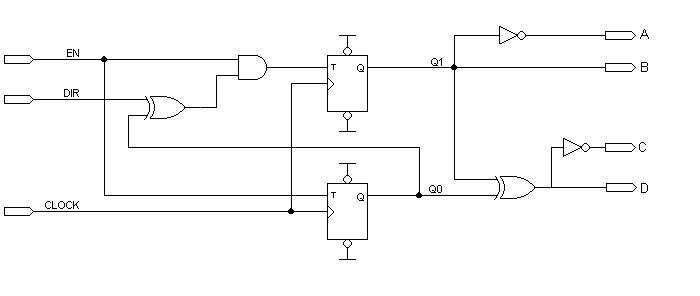
\includegraphics[width=13.778cm,height=5.817cm]{./images/FSM-img9.png} \par}

{\centering Figura 9. Diagrama a nivel de compuertas del controlador de Motor de Paso.\par}

Como puede observarse en la Figura 9, la máquina de estados está formada por la lógica de estado siguiente (Compuertas XOR y AND), la memoria de
estado (FFs tipo T con la misma señal de Reloj) y la lógica de salida, (Compuertas NOT y XOR) que en este caso corresponde al de una máquina de estados tipo MOORE.


{\centering 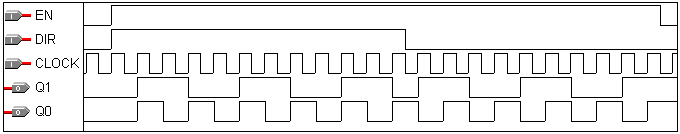
\includegraphics[width=14.984cm,height=2.953cm]{./images/FSM-img10.png} \par}

{\centering Figura 10. Simulación del Controlador de Motor de Paso. \par}

\subsection[DESCRIPCION VHDL DE UNA FSM]{ DESCRIPCION VHDL DE UNA FSM}

En esta sección se realizará la descripción en VHDL del controlador de motor de paso. Inicialmente se hará una descripción estructural, basándose en los resultados obtenidos en la sección 5.4.3.7. Y a continuación se utilizará la descripción funcional para la implementación del controlador.

\subsubsection[DESCRIPCION ESTRUCTURAL]{DESCRIPCION ESTRUCTURAL}

Recordemos que la descripción estructural en VHDL realiza la interconexión entre los componentes que forman el sistema. En nuestro caso (Ver Figura 9), primero debemos realizar la descripción de los componentes:

\paragraph[Compuerta AND de dos entradas]{Compuerta AND de dos entradas}
\begin{lstlisting}
ENTITY and2 IS -- Debido a que AND es una palabra reservada del lenguaje
-- no puede utilizarse para nombrar una entidad
PORT(
    A : IN BIT;
    B : IN BIT;
    Y : OUT BIT);
    END and2;
ARCHITECTURE Y OF and2 IS
BEGIN
    Y <= A AND B;
END;
\end{lstlisting}

\paragraph[Compuerta XOR de dos entradas]{Compuerta XOR de dos entradas}
\begin{lstlisting}
ENTITY xor2 IS -- Debido a que XOR es una palabra reservada del lenguaje
-- no puede utilizarse para nombrar una entidad
  PORT(
    A : IN BIT;
    B : IN BIT;
    Y : OUT BIT); 
END xor2;

ARCHITECTURE XR OF xor2 IS
  BEGIN
    Y <= A XOR B;
  END;
\end{lstlisting}

\paragraph[INVERSOR]{ INVERSOR}
\begin{lstlisting}

INVERSOR ENTITY inv IS
  PORT(
    A : IN BIT;
    Y : OUT BIT); 
END inv;
ARCHITECTURE NO OF inv IS
  BEGIN
    Y <= not (A);
  END;
\end{lstlisting}

\paragraph[FLIP FLOP TIPO T]{ FLIP FLOP TIPO T}
\begin{lstlisting}
FLIP FLOP TIPO T ENTITY FFT IS
  PORT(
    T,CLK : IN BIT;
    Q : BUFFER BIT);
END FFT;
ARCHITECTURE T OF FFT IIS
  BEGIN
   process (CLK) begin
    if (CLK'event and CLK = '1') then
     if (t = '1') then
      Q <= not (Q);
     else
      Q <= Q;
     end if;
    end if;
   end process;
  END;
\end{lstlisting}


Una vez realizada la implementación de los componentes, se procede a su unión. Para lograr esto se deben sintetizar las anteriores declaraciones, y sus archivos deben estar en el mismo directorio de trabajo.

\paragraph[CONTROL DE MOTOR DE PASO]{ CONTROL DEMOTOR DE PASO}
\begin{lstlisting}
CONTROL DE MOTOR DE PASO ENTITY StepMotor IS
  PORT(
    CLK, EN, DIR : IN BIT;
    AO, BO, CO, DO : BUFFER BIT);
END StepMotor;

ARCHITECTURE CONTROLLER OF StepMotor IS
  SIGNAL I1, T1, Q0N: BIT;
  COMPONENT AND2E
    PORT (A, B : IN BIT;
             Y : OUT BIT);
  END COMPONENT;
  COMPONENT XOR2
    PORT (A, B : IN BIT;
             Y : OUT BIT);
  END COMPONENT;
  COMPONENT INV
    PORT (A : IN BIT;
          Y : OUT BIT);
  END COMPONENT;
  COMPONENT FFT
    PORT(
    CLK, T: IN BIT;
        Q : OUT BIT);
  END COMPONENT;

  BEGIN
    X1: XOR2 port map(DIR, Q0N, I1);
    X2: AND2E port map(EN, I1, T1);
    X3: FFT port map(CLK, T1, BO);
    X4: FFT port map(CLK, EN, Q0N);
    X5: XOR2 port map(BO, Q0N, DO);
    X6: INV port map(BO, AO);
    X7: INV port map(DO, CO);
  END CONTROLLER;
\end{lstlisting}

\subsubsection[DESCRIPCION FUNCIONAL]{DESCRIPCION FUNCIONAL}

La descripción Estructural no es el mejor ejemplo de la potencialidad del VHDL, ya que como vimos, es necesario realizar todo el proceso de  síntesis para obtener las ecuaciones de excitación de los Flip-Flops. Realizando la descripción funcional no es necesario preocuparse por escoger el Flip -- Flop que reduzca el número de compuertas ni de minimizar las ecuaciones booleanas obtenidas, todos estos procesos los realizan automáticamente las herramientas CAD disponibles comercialmente. El código VHDL del controlador del motor de paso se muestra a continuación, y en la Figura 11 se muestra el resultado de la simulación.


\begin{lstlisting}
library ieee;
USE ieee.std_logic_1164.all;
USE ieee.std_logic_arith.all;

ENTITY FSMF IS
  PORT(
   clk        : IN std_logic;
   EN, DIR    : IN std_logic;
   A, B, C, D : OUT std_logic);
END FSMF;

ARCHITECTURE funcional OF FSMF IS
TYPE estados IS (S1, S2, S3, S4);
SIGNAL state : estados;

BEGIN
  PROCESS (clk)
   BEGIN
    IF (clk'event and clk = '1') then
     case state is
      when S1 => A <= '1'; B <= '0'; C <= '1'; D <= '0';
       IF (EN = '0') then
        state <= S1;
       ELSIF (DIR = '0') then
        state <= S2;
       ELSE
        state <= S4;
       END IF;

      when S2 => A <= '1'; B <= '0'; C <= '0'; D <= '1';
       IF (EN = '0') then
        state <= S2;
       ELSIF (DIR = '0') then
        state <= S3;
       ELSE
        state <= S1;
       END IF;

      when S3 => A <= '0'; B <= '1'; C <= '0'; D <= '1';
       IF (EN = '0') then
        state <= S3;
       ELSIF (DIR = '0') then
        state <= S4;
       ELSE
        state <= S2;
       END IF;
      when S4 => A <= '0'; B <= '1'; C <= '1'; D <= '0';
       IF (EN = '0') then
        state <= S4;
       ELSIF (DIR = '0') then
        state <= S1;
       ELSE
        state <= S3;
      END IF;
     END CASE;
    END IF;
  END PROCESS;
END funcional;
\end{lstlisting}







{
El código para la realización del Test Bench es:}

{\itshape
\textbf{LIBRARY} ieee;}

{\itshape
\textbf{USE} ieee.std\_logic\_1164.ALL;}

{\itshape
\textbf{USE} ieee.numeric\_std.ALL;}

{\itshape
\textbf{ENTITY} testbench \textbf{IS}}

{\itshape
\textbf{END} testbench;}

{\itshape
\textbf{ARCHITECTURE} behavior \textbf{OF} testbench \textbf{IS} }

{\itshape
\ \ \textbf{COMPONENT} fsmf}

{\itshape
\ \ \textbf{PORT}(}

{\itshape
\ \ \ \ clk : \textbf{IN} std\_logic;}

{\itshape
\ \ \ \ EN : \textbf{IN} std\_logic;}

{\itshape
\ \ \ \ DIR : \textbf{IN} std\_logic;  }

{\itshape
\ \ \ \ A : \textbf{OUT} std\_logic;}

{\itshape
\ \ \ \ B : \textbf{OUT} std\_logic;}

{\itshape
\ \ \ \ C : \textbf{OUT} std\_logic;}

{\itshape
\ \ \ \ D : \textbf{OUT} std\_logic}

{\itshape
\ \ \ \ );}

{\itshape
\ \ \textbf{END} \textbf{COMPONENT};}

{\itshape
\ \ \textbf{SIGNAL} clk :  std\_logic;}

{\itshape
\ \ \textbf{SIGNAL} EN :  std\_logic;}

{\itshape
\ \ \textbf{SIGNAL} DIR :  std\_logic;}

{\itshape
\ \ \textbf{SIGNAL} A :  std\_logic;}

{\itshape
\ \ \textbf{SIGNAL} B :  std\_logic;}

{\itshape
\ \ \textbf{SIGNAL} C :  std\_logic;}

{\itshape
\ \ \textbf{SIGNAL} D :  std\_logic;}

{\itshape
 \textbf{constant} ncycles  : \textbf{integer} := 40;}

{\itshape
 \textbf{constant} halfperiod : \textbf{time  } := 5 ns;}

{\bfseries\itshape
BEGIN}

{\itshape
 \ \ uut: fsmf \textbf{PORT} \textbf{MAP}(}

{\itshape
\foreignlanguage{english}{\ \ \ \ }\foreignlanguage{spanish}{clk
={\textgreater} clk,}}

{\itshape
\ \ \ \ EN ={\textgreater} EN,}

{\itshape
\ \ \ \ DIR ={\textgreater} DIR,}

{\itshape
\ \ \ \ A ={\textgreater} A,}

{\itshape
\foreignlanguage{spanish}{\ \ \ \ }\foreignlanguage{english}{B
={\textgreater} B,}}

{\itshape
\ \ \ \ C ={\textgreater} C,}

{\itshape
\foreignlanguage{english}{\ \ \ \ }\foreignlanguage{spanish}{D
={\textgreater} D);}}

{\itshape
 {}-{}- Generacion del Reloj}

{\itshape
\foreignlanguage{spanish}{ }\foreignlanguage{english}{Clock\_Source:
}\foreignlanguage{english}{\textbf{process}}}

{\itshape
 \textbf{begin}}

{\itshape
 \textbf{for} i \textbf{in} 0 \textbf{to} ncycles \textbf{loop}  {}-{}-
Genera ncyclos de periodo 10 ns}

{\itshape
 clk {\textless}= {\textquotesingle}0{\textquotesingle};}

{\itshape
 \textbf{wait} \textbf{for} halfperiod;}

{\itshape
 clk {\textless}= {\textquotesingle}1{\textquotesingle};}

{\itshape
 \textbf{wait} \textbf{for} halfperiod;}

{\itshape
 \textbf{end} \textbf{loop};}

{\itshape
 \textbf{wait};}

{\itshape
 \textbf{end} \textbf{process} Clock\_Source;}

{\itshape
 tb : PROCESS}

{\itshape
\ \ \textbf{BEGIN}}

{\itshape
 \textbf{for} i \textbf{in} 1 \textbf{to} ncycles/4 \textbf{loop 
}{}-{}- Durante ncyclos/4 genera las diferentes}

{\itshape
\foreignlanguage{english}{
}\foreignlanguage{spanish}{\textbf{wait}}\foreignlanguage{spanish}{
}\foreignlanguage{spanish}{\textbf{until}}\foreignlanguage{spanish}{
Clk={\textquotesingle}1{\textquotesingle}
}\foreignlanguage{spanish}{\textbf{and}}\foreignlanguage{spanish}{
Clk}\foreignlanguage{spanish}{\textbf{{\textquotesingle}event}}\foreignlanguage{spanish}{;
 {}-{}- Combinaciones de EN y DIR}}

{\itshape
 EN  {\textless}= {\textquotesingle}0{\textquotesingle};}

{\itshape
\foreignlanguage{spanish}{ }\foreignlanguage{english}{DIR {\textless}=
{\textquotesingle}0{\textquotesingle};}}

{\itshape
 \textbf{end} \textbf{loop};}

{\itshape
 \textbf{for} i \textbf{in} 1 \textbf{to} ncycles/4 \textbf{loop}}

{\itshape
 \textbf{wait} \textbf{until} Clk={\textquotesingle}1{\textquotesingle}
\textbf{and} Clk{\textquotesingle}\textbf{event};}

{\itshape
\foreignlanguage{english}{ }\foreignlanguage{spanish}{EN  {\textless}=
{\textquotesingle}0{\textquotesingle};}}

{\itshape
\ \   DIR {\textless}= {\textquotesingle}1{\textquotesingle};}

{\itshape
\foreignlanguage{spanish}{
}\foreignlanguage{english}{\textbf{end}}\foreignlanguage{english}{
}\foreignlanguage{english}{\textbf{loop}}\foreignlanguage{english}{; 
}}

{\itshape
 \textbf{for} i \textbf{in} 1 \textbf{to} ncycles/4 \textbf{loop}}

{\itshape
 \textbf{wait} \textbf{until} Clk={\textquotesingle}1{\textquotesingle}
\textbf{and} Clk{\textquotesingle}\textbf{event};}

{\itshape
\foreignlanguage{english}{ }\foreignlanguage{spanish}{EN  {\textless}=
{\textquotesingle}1{\textquotesingle};}}

{\itshape
\ \   DIR {\textless}= {\textquotesingle}0{\textquotesingle};}

{\itshape
\foreignlanguage{spanish}{
}\foreignlanguage{english}{\textbf{end}}\foreignlanguage{english}{
}\foreignlanguage{english}{\textbf{loop}}\foreignlanguage{english}{; 
\ \  }}

{\itshape
 \textbf{for} i \textbf{in} 1 \textbf{to} ncycles/4 \textbf{loop}}

{\itshape
 \textbf{wait} \textbf{until} Clk={\textquotesingle}1{\textquotesingle}
\textbf{and} Clk{\textquotesingle}\textbf{event};}

{\itshape
\foreignlanguage{english}{ }\foreignlanguage{spanish}{EN  {\textless}=
{\textquotesingle}1{\textquotesingle};}}

{\itshape
\ \   DIR {\textless}= {\textquotesingle}1{\textquotesingle};}

{\itshape
\foreignlanguage{spanish}{
}\foreignlanguage{english}{\textbf{end}}\foreignlanguage{english}{
}\foreignlanguage{english}{\textbf{loop}}\foreignlanguage{english}{; 
}}

{\itshape
 \textbf{END} \textbf{PROCESS};}

{\itshape
\textbf{END};}

 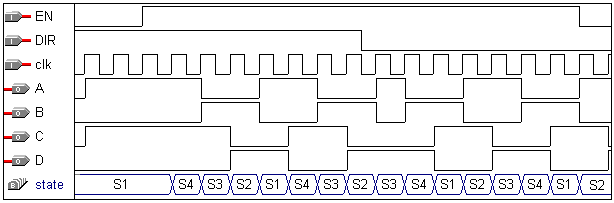
\includegraphics[width=13.286cm,height=4.382cm]{./images/FSM-img11.png} 

{\centering
Figura 11. Simulación de la descripción funcional del controlador de
motor de paso.
\par}

{
Con la descripción funcional no es necesario preocuparse por el tipo de
Flip-Flop ni por los procesos de minimización.}

{
Normalmente las herramientas CAD proporcionan información sobre
resultado de ls síntesis del diseño, las ecuaciones implementadas en un
CPLD por una de estas herramientas es:}

{\itshape
clk  : INPUT;}

{\itshape
DIR  : INPUT;}

{\itshape
EN  : INPUT;}

{\itshape
A  = DFFE( state\~{}2 \$  VCC,  GLOBAL( clk),  VCC,  VCC,  VCC);}

{\itshape
B  = DFFE(!state\~{}2 \$  VCC,  GLOBAL( clk),  VCC,  VCC,  VCC);}

{\itshape
C  = DFFE(!state\~{}1 \$  state\~{}2, GLOBAL( clk),  VCC,  VCC,  VCC);}

{\itshape
D  = DFFE( state\~{}1 \$  state\~{}2, GLOBAL( clk),  VCC,  VCC,  VCC);}

{\bfseries\itshape
state\~{}1  = TFFE( EN, GLOBAL( clk),  VCC,  VCC,  VCC);}

{\bfseries\itshape
state\~{}2  = TFFE( \_EQ001, GLOBAL( clk),  VCC,  VCC,  VCC);}

{\itshape
\foreignlanguage{english}{\textbf{
}}\foreignlanguage{spanish}{\textbf{\_EQ001 = !DIR \&  EN \& 
state\~{}1  \#  DIR \&  EN \&
!state\~{}1}}\foreignlanguage{spanish}{;}}

{
En donde se puede observar que se llegó a las mismas ecuaciones
obtenidas anteriormente. Observe que se utilizaron 2 Flip-Flops tipo T
uno de los cuales tiene a la señal EN como entrada (primera seña que
aparece dentro de los paréntesis después de TFFE. ). Mientras que el
otro tiene a la señal \_EQ001 conectada a su entrada T. La ecuación
para \_EQ001 es:}

{
 \textit{!DIR \&  EN \&  state\~{}1  \#  DIR \&  EN \& !state\~{}1 =
EN.((!DIR.sate\~{}1) + (DIR.!state\~{}1)}}

{
Como vimos en capítulos anteriores la arquitectura de un CPLD no posee
compuertas XOR, por lo tanto las ecuaciones son de la forma de suma de
productos. Lo interesante es observar el ahorro de tiempo asociado a la
utilización del VHDL como herramienta de diseño.}

